
\section{Architecture Integration}

\subsection{Model Support Matrix}

\begin{table}[H]
\centering
\small
\begin{tabular}{llllll}
\toprule
\textbf{Architecture} & \textbf{Attention} & \textbf{Nested?} & \textbf{RoPE?} & \textbf{GQA?} & \textbf{Galerkin path?} \\
\midrule
DistilBERT & \texttt{MultiHeadSelfAttention} & No & No & No & (encoder) \\
RoBERTa & \texttt{BertSelfAttention} & Yes & No & No & (encoder) \\
GPT-2 & \texttt{GPT2Attention} & No & No & No & (decoder fallback) \\
Qwen3.5 & \texttt{Qwen3Attention} & No & Yes & Yes & (decoder fallback) \\
\bottomrule
\end{tabular}
\end{table}

\subsection{Weight Transfer}

\subsubsection{Conv1D Orientation (GPT-2)}

HuggingFace \texttt{Conv1D} stores \texttt{(in, out)}; we transpose to \texttt{(out, in)}:

\begin{lstlisting}
if "Conv1D" in cls_c or hasattr(c_attn_mod, "nf"):
    c_w = c_w.t()
\end{lstlisting}

We detect via class name \textbf{or} shape heuristic \texttt{w.shape[0] < w.shape[1]}.

\subsubsection{Nested Encoder Detection (RoBERTa)}

The detection order matters. We check \texttt{out\_lin} \textbf{first}:

\begin{lstlisting}
has_out_lin = hasattr(src, "out_lin") or hasattr(src, "c_proj") or hasattr(src, "o_proj")

if has_out_lin:
    is_nested = False     # DistilBERT has out_lin inside attention
elif (hasattr(src, "self") and hasattr(src.self, "query")
      and hasattr(src, "output") and hasattr(src.output, "dense")):
    is_nested = True      # RoBERTa
elif cls_name in ["BertSelfAttention", "RobertaSelfAttention"]:
    is_nested = True
else:
    is_nested = False
\end{lstlisting}

\textbf{Critical bug avoided.} DistilBERT's \texttt{MultiHeadSelfAttention} ends with 
"SelfAttention" and would be misclassified as nested if we did not check 
\texttt{out\_lin} first.

\subsubsection{GQA Support}

For Qwen with $H_{kv} < H$:

\begin{lstlisting}
if self.num_kv_heads != self.num_heads:
    K = repeat_kv(K, self.kv_repeat)
    V = repeat_kv(V, self.kv_repeat)
\end{lstlisting}

\texttt{repeat\_kv} broadcasts and reshapes:

\begin{lstlisting}
def repeat_kv(x, n_rep):
    B, H_kv, N, d = x.shape
    x = x[:, :, None, :, :].expand(B, H_kv, n_rep, N, d)
    return x.reshape(B, H_kv * n_rep, N, d)
\end{lstlisting}

\subsection{Injection Algorithm}

\textbf{Algorithm 2:} Inject Galerkin Attention
\begin{lstlisting}
Input:  layer  , config, old_attn
Output: new attention in  

 1: new $\leftarrow$ GalerkinAttention(config, old_attn=old_attn)
 2: if copy_weights fails: return None
 3: if   has .attention.self:
 4:      .attention.self $\leftarrow$ new
 5:     new.is_nested_encoder $\leftarrow$ True
 6: elif   has .attention:
 7:      .attention $\leftarrow$ new
 8: elif   has .attn:
 9:      .attn $\leftarrow$ new
10: elif   has .self_attn:
11:      .self_attn $\leftarrow$ new
12: return new
\end{lstlisting}

\subsection{Causal Handling}

The \texttt{is\_decoder} flag determines which path is taken:

\begin{lstlisting}
is_dec = (
    getattr(config, "is_decoder", False)
    or getattr(config, "is_causal", False)
    or any(_mt.startswith(p) for p in ("gpt", "qwen", "llama", "mistral"))
)
\end{lstlisting}

For GPT-2 and Qwen, \texttt{is\_decoder=True} and the fallback path is taken.

\subsection{RoPE Support}

Galerkin Attention handles partial RoPE via dimension slicing:

\begin{lstlisting}
rotary_dim = cos.shape[-1]
if rotary_dim < head_dim:
    q_rot, q_pass = q[..., :rotary_dim], q[..., rotary_dim:]
    q_rot_embed = q_rot * cos + rotate_half(q_rot) * sin
    q = torch.cat([q_rot_embed, q_pass], dim=-1)
\end{lstlisting}

\subsection{Failure Handling}

\begin{table}[H]
\centering
\small
\begin{tabular}{lll}
\toprule
\textbf{Failure} & \textbf{Detection} & \textbf{Response} \\
\midrule
Weight copy failure & Frobenius < 1e-4 & Log warning \\
Missing projection & \texttt{missing\_after} non-empty & Log warning \\
Basis QR failure & try/except & Fallback \\
Cross-attention & \texttt{encoder\_hidden\_states != None} & Not supported \\
\bottomrule
\end{tabular}
\end{table}

\subsection{Registry}

\begin{lstlisting}
@ATTENTION_REGISTRY.register("galerkin")
@ATTENTION_REGISTRY.register("galerkin_attention")
class GalerkinAttention(BaseAttention):
    ...
\end{lstlisting}

\subsection{Common Pitfalls}

\subsubsection{Basis Rebuild per Forward}

The basis $\Phi$ is rebuilt on every forward call because it depends on 
$N = $ sequence length. For a fixed $N$, this is wasteful. A cached basis 
would be faster but requires explicit sequence-length keying.

\subsubsection{Fixed Basis Cannot Adapt}

The DCT basis is data-independent. It cannot learn to attend to specific 
positions or content. This is the root cause of the negative results.

\subsubsection{Nested Encoder Double-Projection}

If \texttt{is\_nested\_encoder} is wrong, the output projection is applied twice 
(once inside our module, once by the outer block).



\begin{figure}[H]
\centering
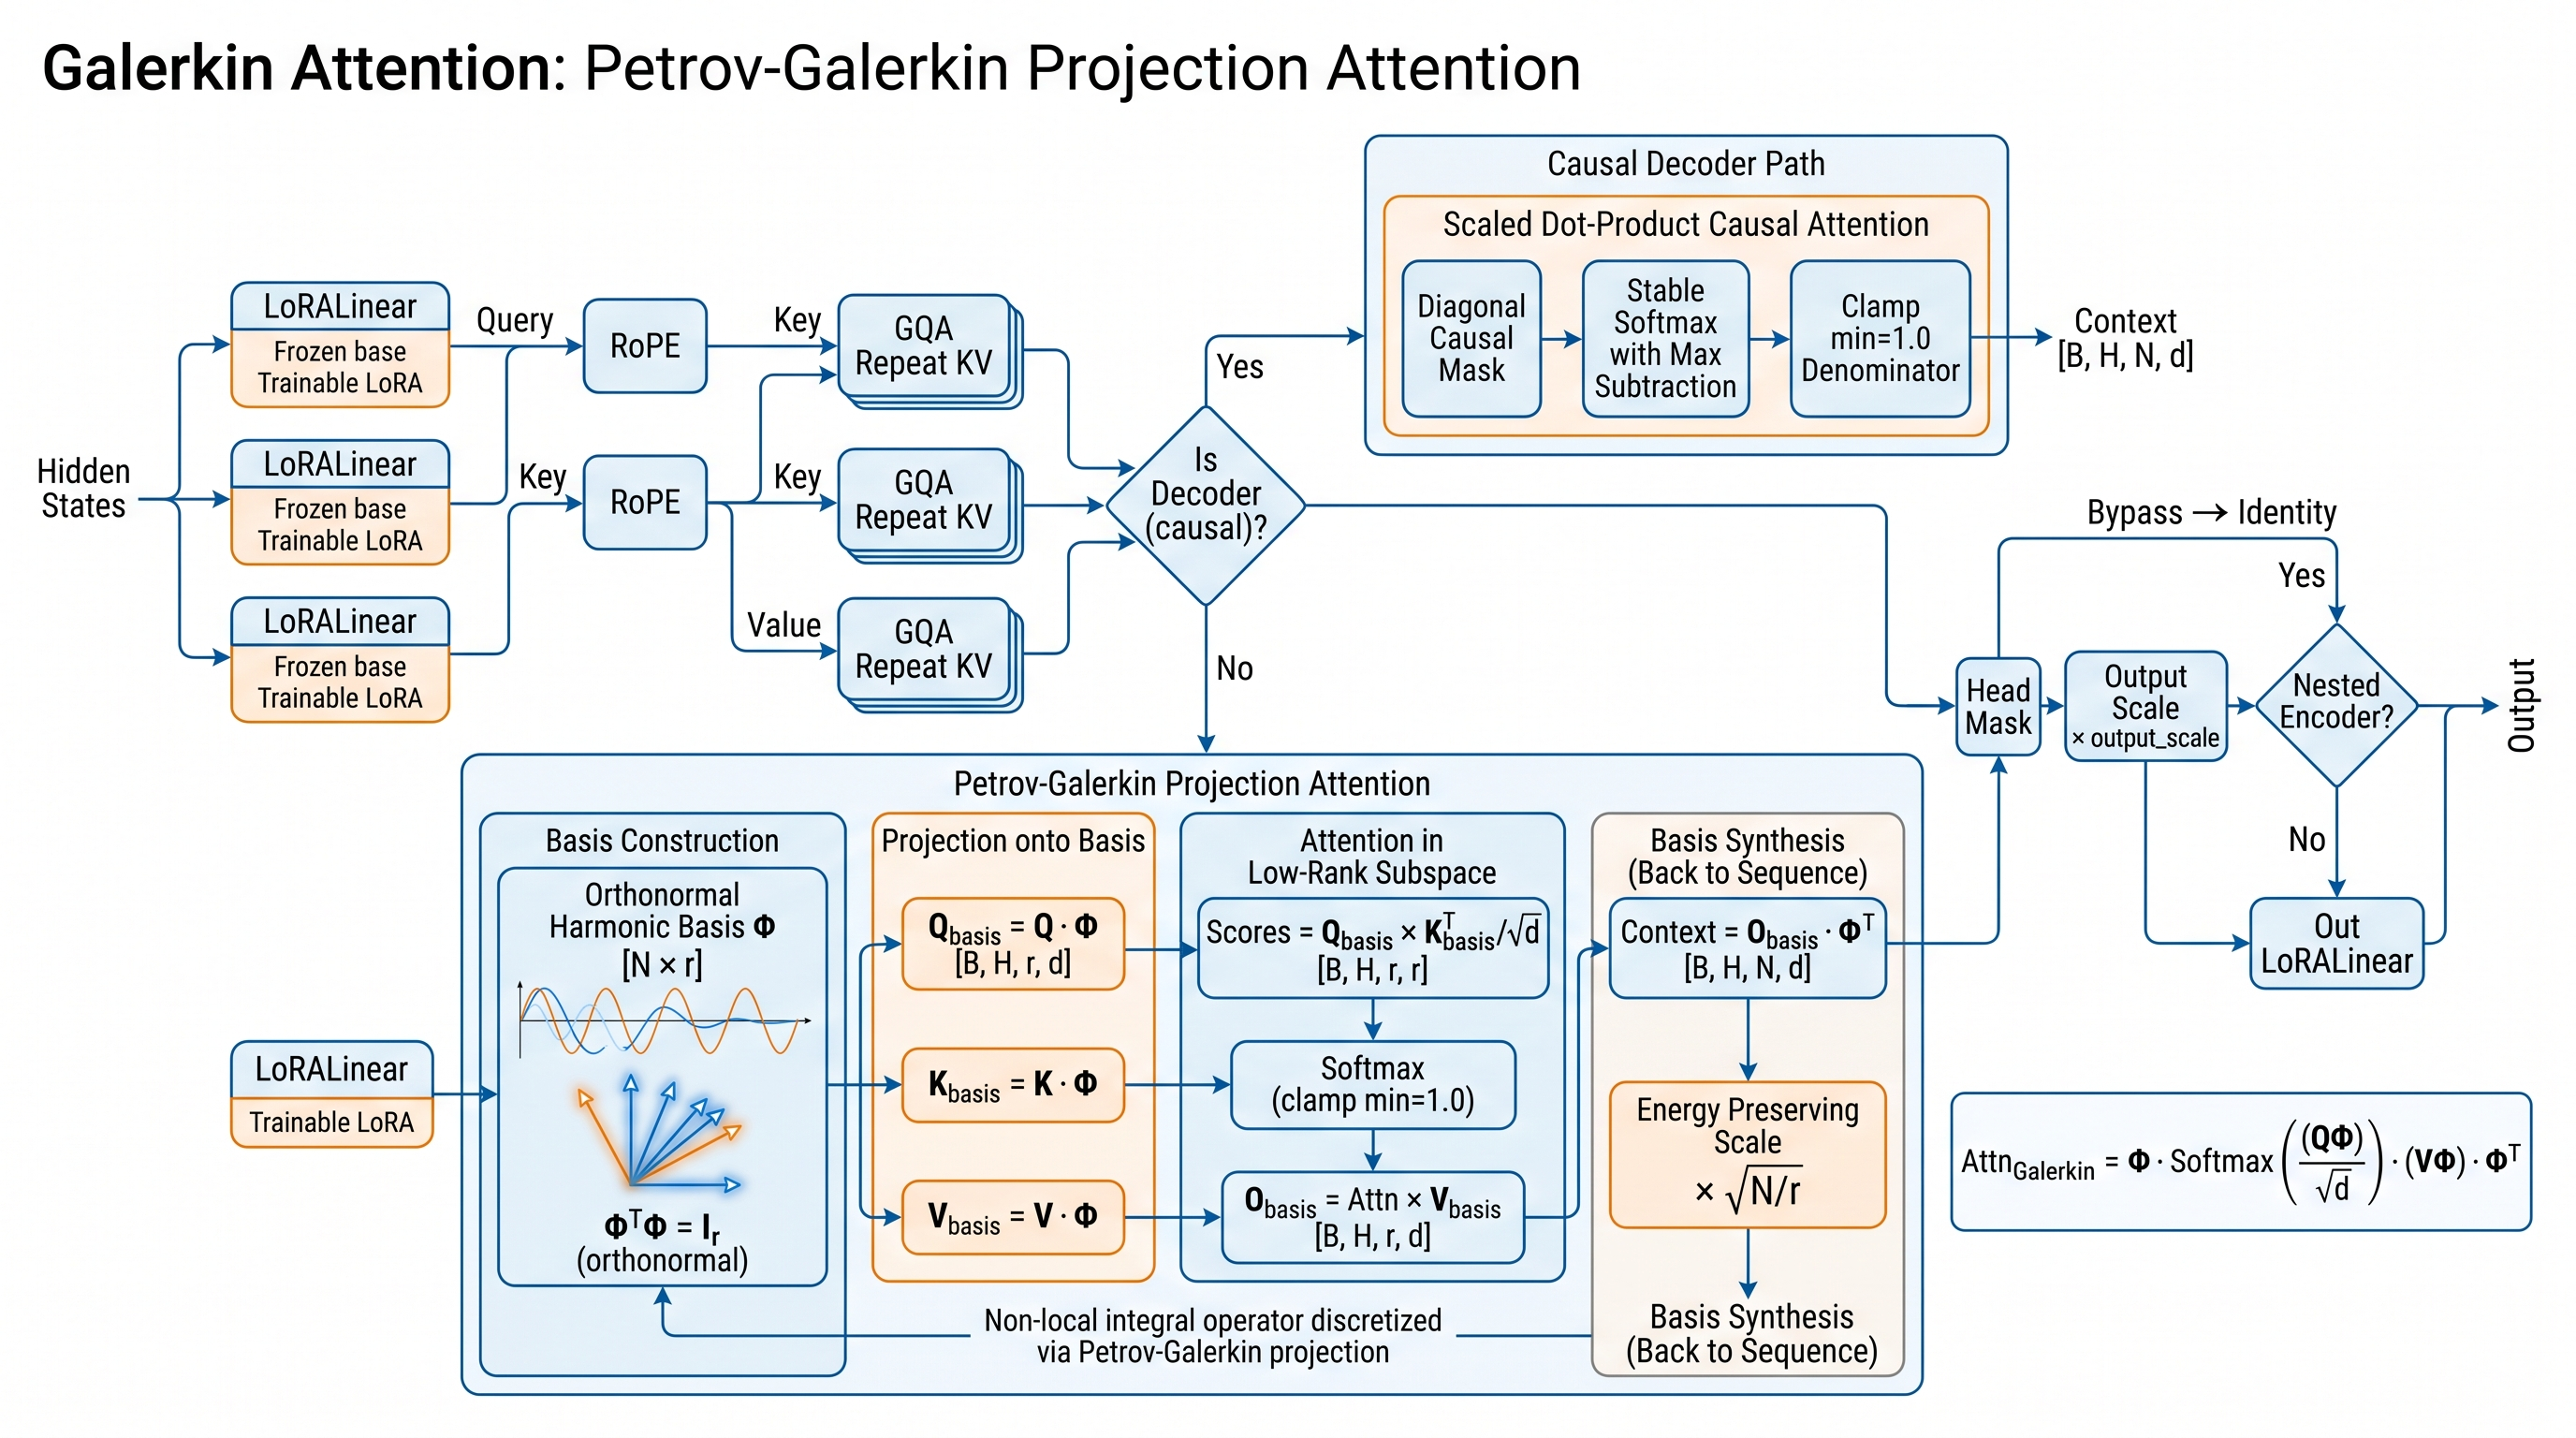
\includegraphics[width=\linewidth]{figures/architecture.jpeg}
\caption{High-level architectural diagram of Galerkin.}
\label{fig:arch_Galerkin}
\end{figure}

